\documentclass{report}
\usepackage{cours}

\linespread{1.2}

\title{Optimization of simplified calculation methods for early age cracking assessment}
\author{Edgar Pierre BURKHART}
\date{2020}

\bibliography{bib}

\begin{document}

\maketitle

\tableofcontents
%%%


\chapter{Literrature review}

\section{Introduction}

Cracking control is a critical point in the design of concrete structures.
Uncontrolled cracking can have a major impact on the durability of reinforced
concrete structures, for several reasons including corrosion of metal rods.
For this reason, the risks of cracking during the early age of a structure have
been studied by numerous research teams in the past. In this chapter, the
results that have been found regarding the evaluation of cracking risks will be
observed.

\section{Creep, Shrinkage and Cracking of Restrained Concrete at Early Age
\cite{cscea}}
\subsection{Introduction}
In 2001, a research team from the University of Illinois realised an
experimental study of the impact of creep and shrinkage on cracking of
restrained concrete regarding various parameters.

\subsection{Methods}
An experimental study was conducted using a uniaxial restrained shrinkage test.
A combination of restrained and unrestrained specimens was used to extract
creep from the results. According to the authors, the difference in strain
between free shrinkage and restrained tests was the creep strain, as seen in
\autoref{aci1}. The experiment's goal was to determine a number of properties
of concrete at early age.

This study was conducted with both normal and high performance concrete as
well as plain and fiber reinforced concrete. The aggregates used were always
the same, and both steel fibers and polypropylene fibers were used in fiber
reinforced concrete. The impact of water to concrete ratio was studied, at
static temperature and humidity values, with two different drying environements
being used.

\begin{figure}
  \centering
  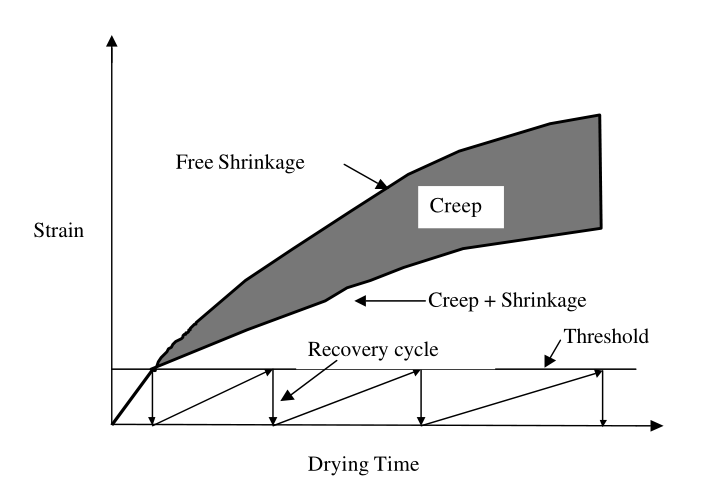
\includegraphics[width=.5\linewidth]{fig/aci1}
  \caption{Schematic diagram of the test mechanism \cite{cscea}.}\label{aci1}
\end{figure}

\subsection{Results}
According to the free shrinkage study, a first stage in which no shrinkage is
experienced by the concrete seems to occur, which is supposed to be caused by
evaporative cooling of the concrete specimens leading to a slight expansion of
the specimens. In the first 10 hours of the study, expansion or shrinkage could
occur depending on the sample.



%\section{Estimation of cracking risk}
%Several methods have been established in order to estimate the cracking risk of
%concrete elements. In this section will be reviewed several methods used in
%previous research.
%
%In 2004, a state-of-the-art report on the control of early age cracking was
%conducted by a team from the Japan Concrete Institute \cite{soa}. The goal of
%this paper was to review existing research on the causes of cracking and
%methodologies used to control this phenomenon.
%
%According to this document, cracking is mainly caused by different types of
%deformation, citing the main causes of those to be autogenous shrinkage, drying
%shrinkage and thermal shrinkage. Although both represent a variation in
%relative humidity, they are still separate phenomenons.
%Autogenous shrinkage defines the decrease in
%material volume due to hydration of cement, while drying shrinkage represents
%the volume changed caused by water evaporation in the concrete.
%Thermal shrinkage is caused by the variations in temperature in the concrete
%caused by the heat generated by the chemical reaction of cement hydration.
%
%It is also pointed that the resulting strain which should be considered is the
%result of a combination of elastic strain, the effects of creep, of autogenous
%and drying shrinkage, as well as thermal shrinkage, and proposes an equation
%defining the total strain as the sum of all strains.
%
%This study also focuses on the characteristics of concrete that matter in
%cracking control, and shows the importance of using the correct elastic modulus
%and strength in order not to overestimate the cracking risk. It also emerges
%from several studies that the specific tensile creep is different from the
%specific compressive creep, but their doesn't seem to be a consensus on how to
%determine it accurately. It also appears that the linear expansion coefficient
%was highly time dependent, and was generally higher at early age.
%
%Multiple analytical models are also presented for the differents aspects of
%this type of study, as using the Burgers model to study elastic and creep
%strain for instance.
%
%Several methods of cracking behavior testing are also discussed, highlighting
%the different experimental approaches possible. A criteria on crack initiation
%is also established, allowing for adapted material choices in concrete
%structures designing.
%
%Other studies have been conducted in order to investigate the effects of
%shrinkage and creep in concrete, as in 2001 by a team of the University of
%Illinois \cite{cscea}. Several tests were conducted, using a combination of a
%restrained shrinkage test and a free shrinkage test to be able to extract the
%creep strain from the experimental study. Their findings show that the history
%of stress evolution has a major impact on crack developement. It is also
%highlighted that the cracking stress is generally lower than the static tensile
%stress, at around \SI{80}{\percent} of the latter. The importance of creep is
%also exposed, displaying a creep to shrinkage ratio of over \SI{50}{\percent}.
%
%On the subject of fiber reinforced concrete, the study shows a delay on the
%appearance of cracks with the addition of fibers, linking these results to a
%likely change in drying creep mechanisms.
%
%In 2008, the Japan Concrete Institue also released updated guidelines on
%cracking control \cite{jci}. The goal of this report was to provide updated
%simplified equations to estimate the cracking risk in concrete structures.
%Using a combination of finite-element modeling and experimental data, simple
%equations are provided which can be used to determine cracking risks and to
%predict the crack width.
%
%The CIRIA also released a guide on thermal crack control in 2011 \cite{ciria}.
%According to this guide, the main cause of cracks in concrete is the thermal
%behavior of concrete, combined with the presence of restraints, which leads to
%the emergence of stresses which are in part reduced by creep. The report is
%able to produce an equation which allows the determination of the restrained
%strain which depends on the temperature drop, the thermal expansion
%coefficient, a restraint factor and a coefficient which relates to relaxation,
%including creep. The guide then provides an extensive design process relative
%to concrete cracking.


%%%
\printbibliography
\end{document}
